% !TEX root = ../main.tex
%% ---------------------------------------------------------------------------
% 4.2 Examination for convergence rates of quadratic meshfree formulation
%% ---------------------------------------------------------------------------

\subsection{Examination for convergence rates of quadratic meshfree formulation}\label{sec:quadratic}

As stated in Section \ref{sec:error}, only when the order of basis function satisfy the minimum requirement $p\ge3$, can the $L_2$ error of various integral schemes achieves optimal convergence performance $p+1$, otherwise, only $p$th order convergence rate of $L_2$ error can be ensured when $p=2$.
Then two benchmark problems will be adopted to test the above theoretical convergence value.

We consider a 1D cantilever beam as shown in Fig. \ref{fig:5}.
The analytical solution and corresponding boundary conditions are as follows:
\begin{equation}\label{beam_solution}
\begin{cases}
w=\sin x-x\\[2pt]
w(0)=0,\quad \theta(0)=0
\end{cases}
\end{equation}
The material and geometry properties of this problem are: flexural rigidity $D=2\times10^{4}$, Poisson's ratio $\nu=0.3$, length $L=10$.
The left boundary is subject to displacement and rotation boundary conditions, which are imposed by Nitsche's method.
Six regular meshfree discretizations with $11$, $21$, $41$, $81$, $161$, $321$ nodes are adopted to observe the convergence performance.
For quadratic meshfree computation, the normalized support size is set as 2.6.

\begin{figure}[pos=htbp]
\centering
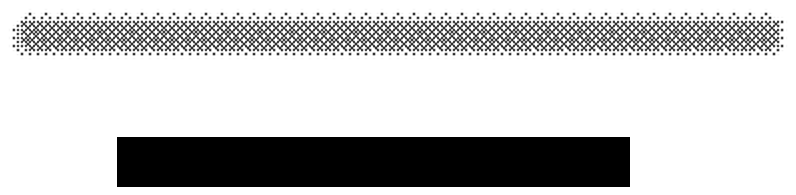
\includegraphics[width=0.7\textwidth]{figs/fig05.png}
\caption{Description of 1D cantilever beam.}\label{fig:5}
\end{figure}

\begin{figure}[pos=htbp]
\centering
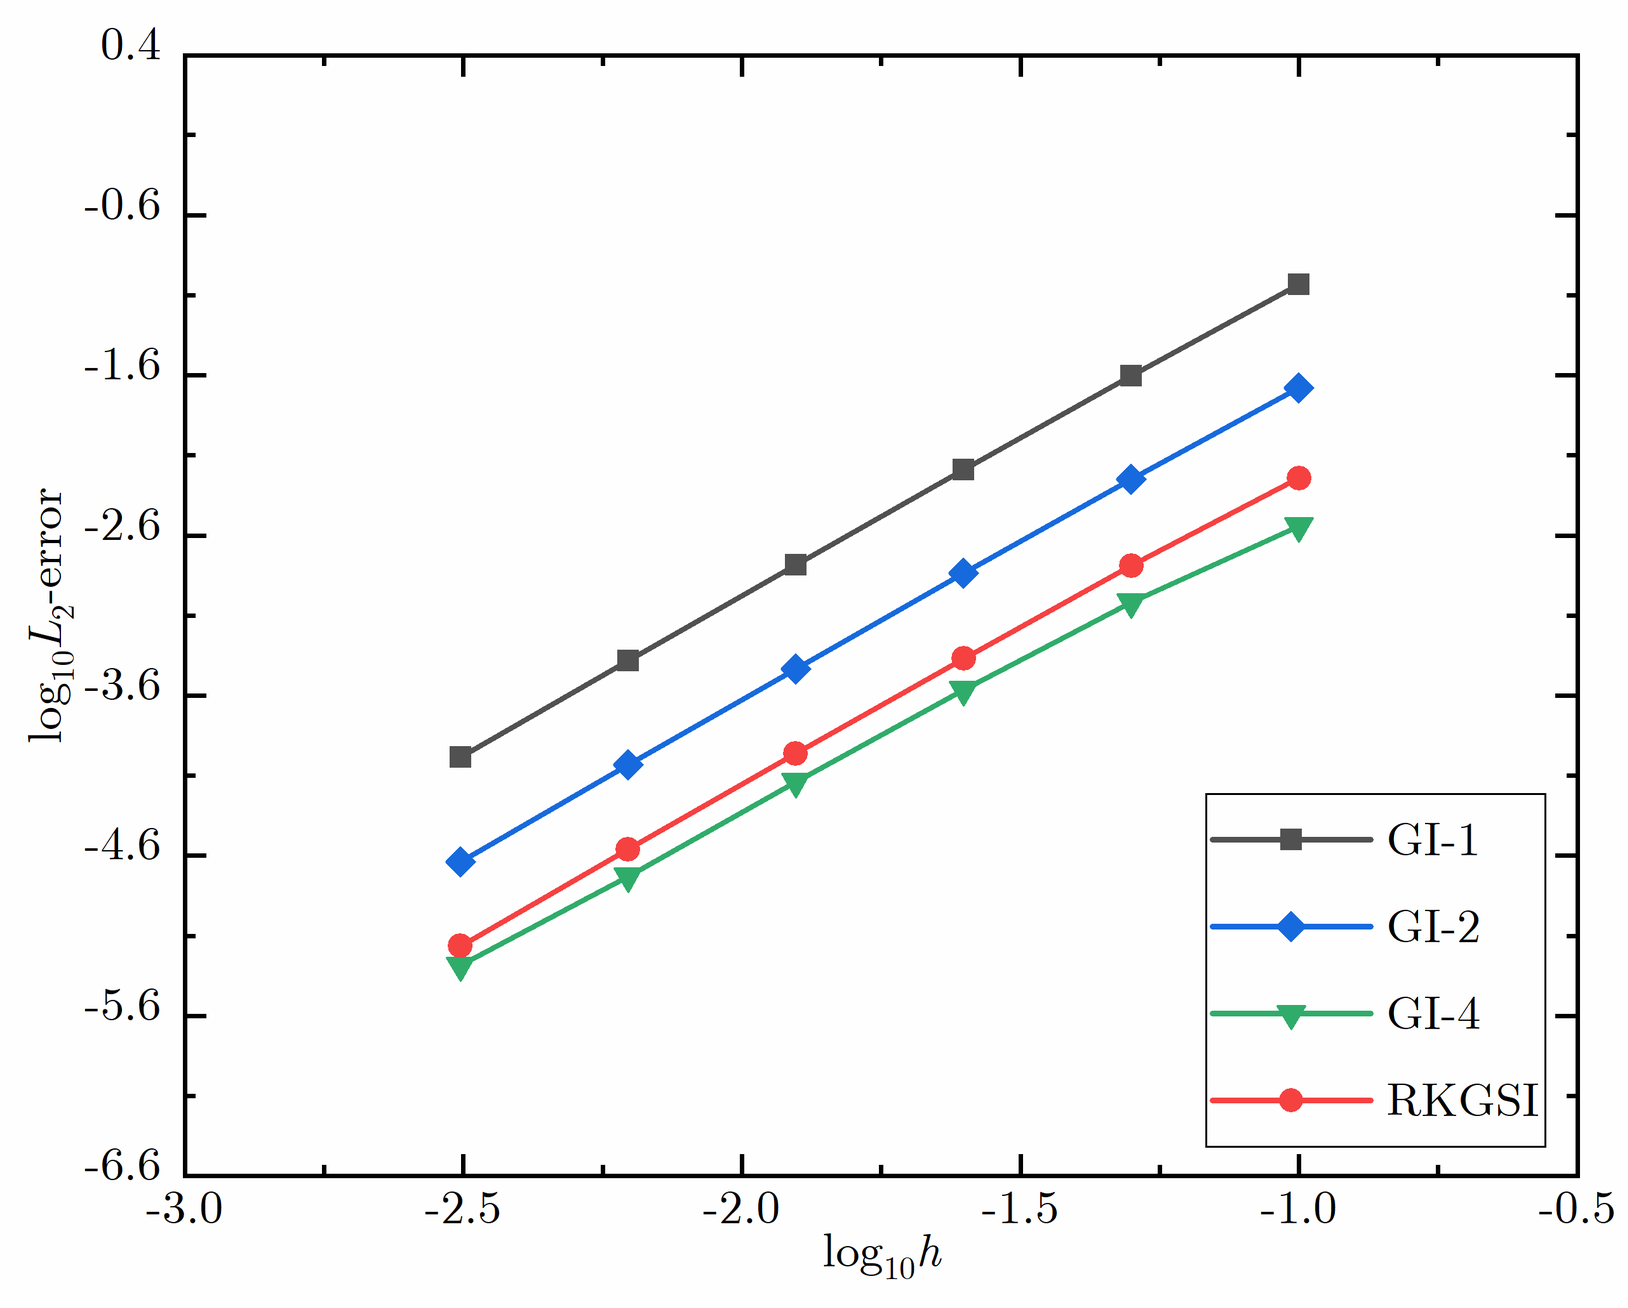
\includegraphics[width=0.55\textwidth]{figs/fig06.png}
\caption{$L_2$-error comparison for the 1D cantilever beam with $p=2$.}\label{fig:6}
\end{figure}

\begin{figure}[pos=htbp]
\centering
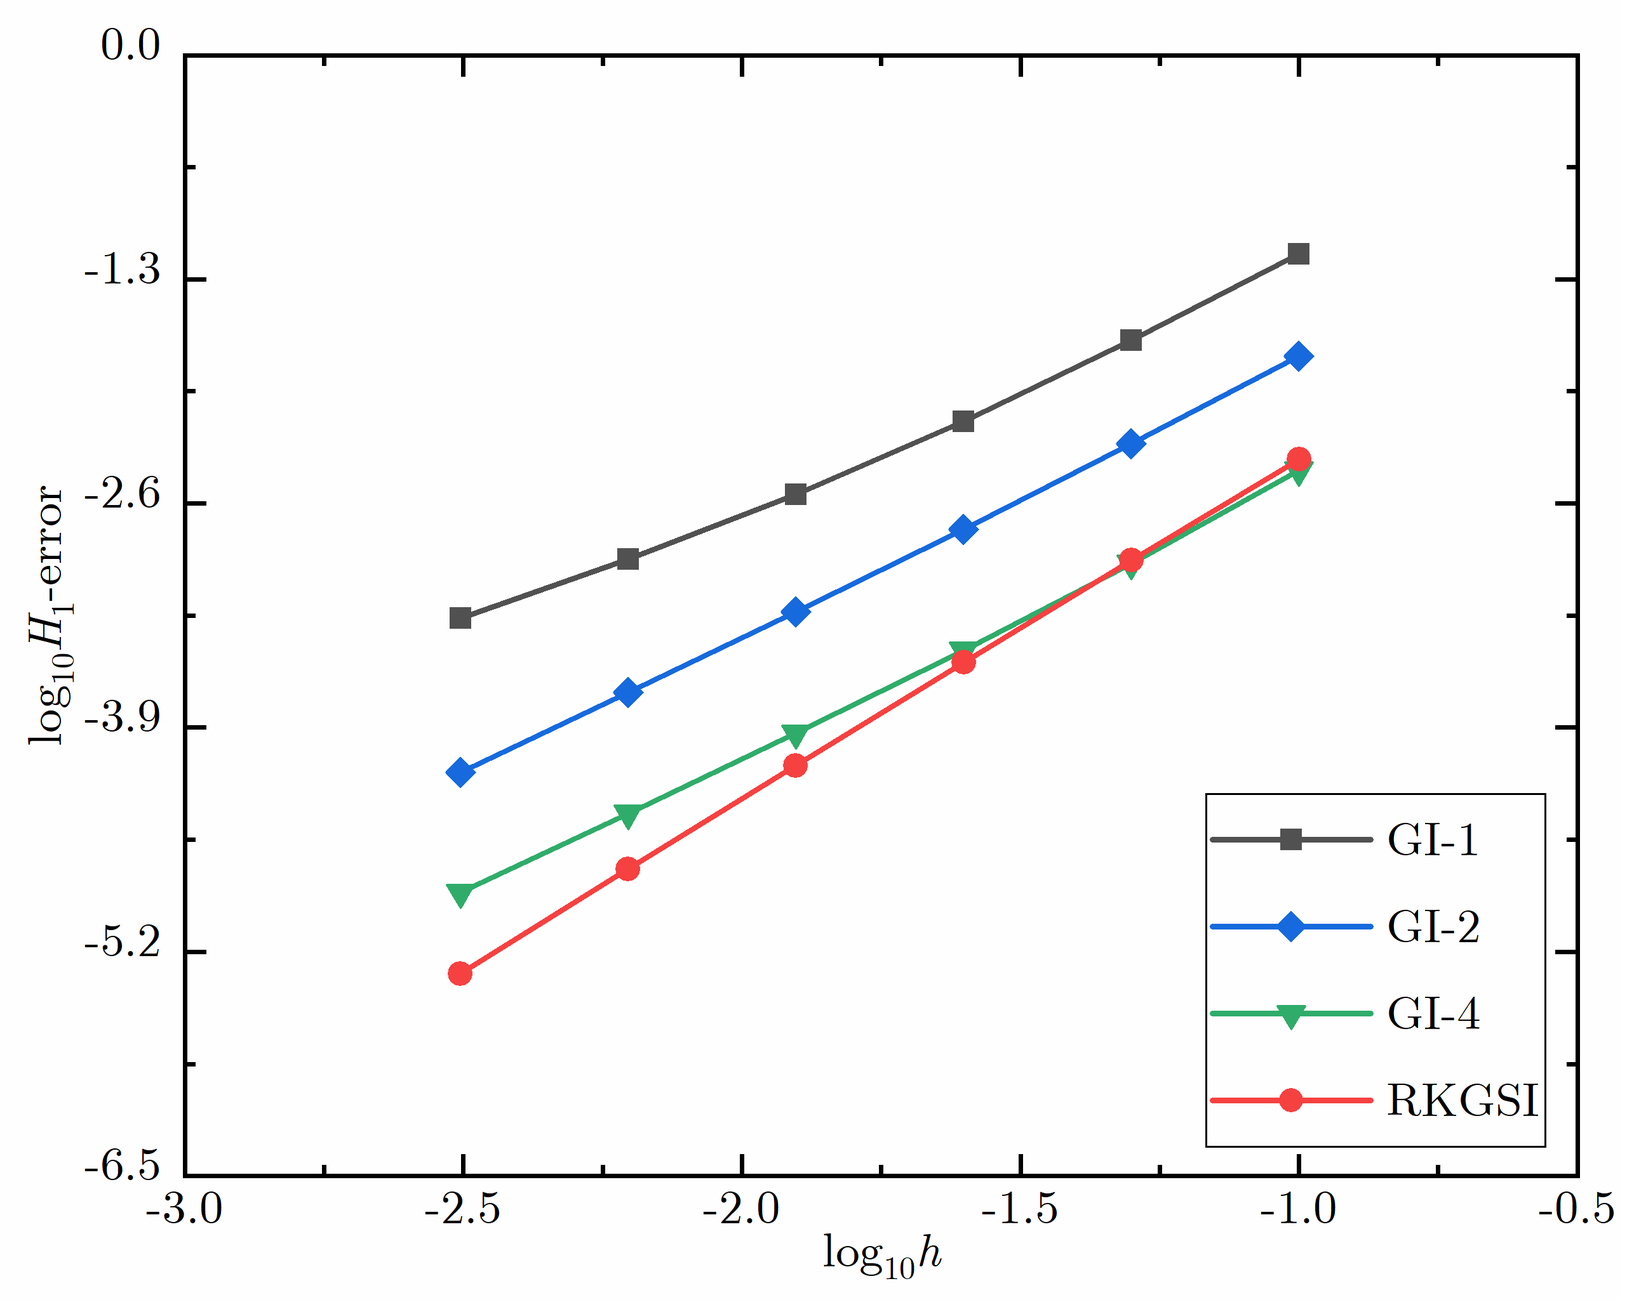
\includegraphics[width=0.55\textwidth]{figs/fig07.png}
\caption{$H_1$-error comparison for the 1D cantilever beam with $p=2$.}\label{fig:7}
\end{figure}

\begin{figure}[pos=htbp]
\centering
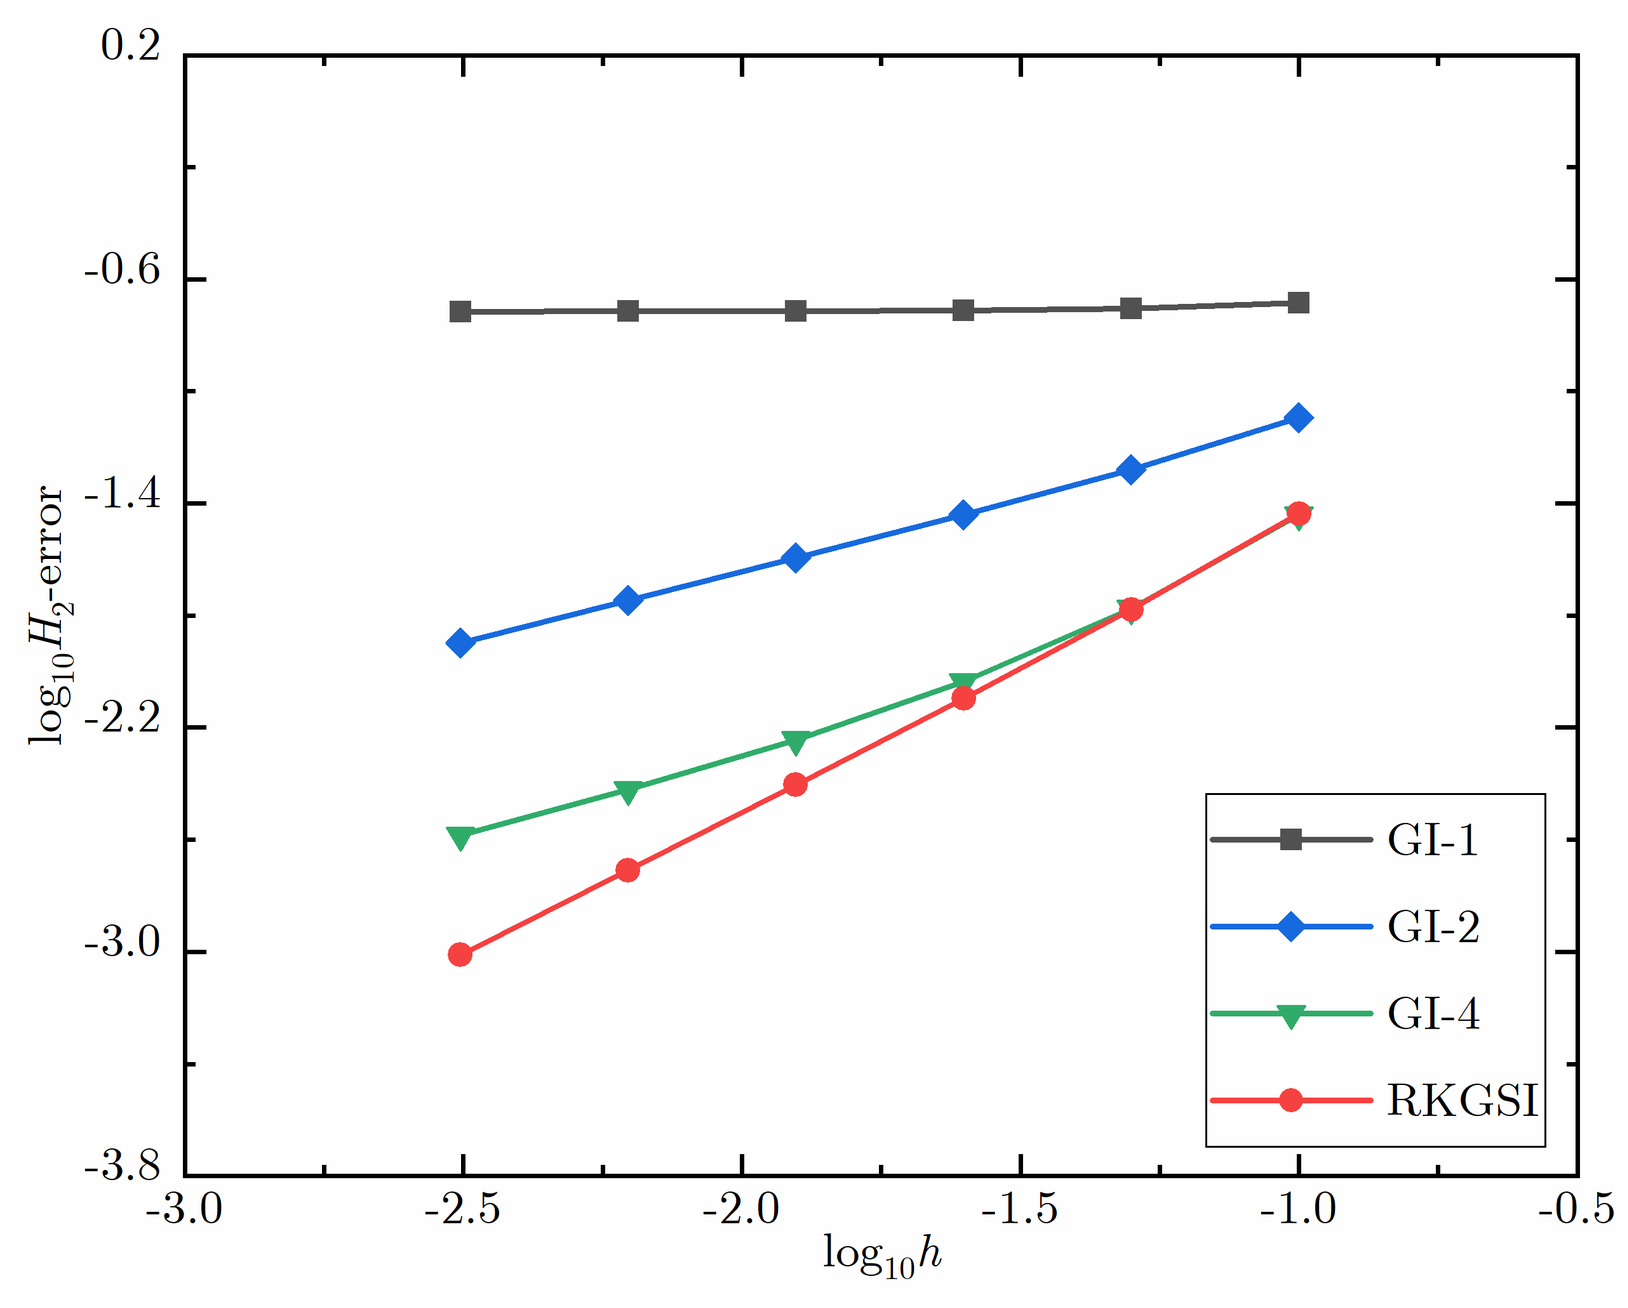
\includegraphics[width=0.55\textwidth]{figs/fig08.png}
\caption{$H_2$-error comparison for the 1D cantilever beam with $p=2$.}\label{fig:8}
\end{figure}

Figs. \ref{fig:6}--\ref{fig:8} show the convergence rates of compute error regarding to $L_2$, $H_1$ and $H_2$ norm for Gauss integration based methods (GI-1, 2, 4) and reproducing kernel gradient smoothing integration based method (RKGSI).
It clearly evinces the importance of the order of basis function, when $p=2$, all the integral schemes both ensure second order of convergence for $L_2$ error even though RKGSI possess the same order of integration consistency as basis function ($q=p=2$), while the integration consistency of GI only be $q=1$.
For $H_1$ and $H_2$ error in Figs. \ref{fig:7} and \ref{fig:8}, notable advantages of RKGSI can be observed with smaller nodal distances, which originates from deficiency of integration consistency of GI.

Another 2D benchmark problem is a left-clamped plate shown in Fig. \ref{fig:9}, whose material properties is the same as the previous 1D beam, geometry property is $L_x=L_y=1$.
The analytical solution and boundary conditions are given by:
\begin{equation}\label{plate_solution}
\begin{cases}
w=\left(\sin x-x\right)\left(y+y^{2}\right)\\[2pt]
w(0,y)=0,\quad \theta(0,y)=0
\end{cases}
\end{equation}

\begin{figure}[pos=htbp]
\centering
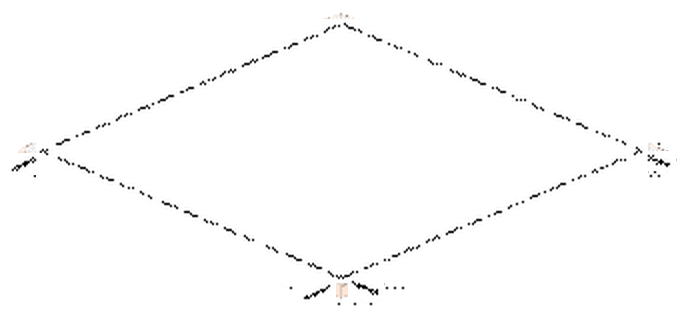
\includegraphics[width=0.6\textwidth]{figs/fig09.png}
\caption{Description of left-clamped plate.}\label{fig:9}
\end{figure}

\begin{figure}[pos=htbp]
\centering
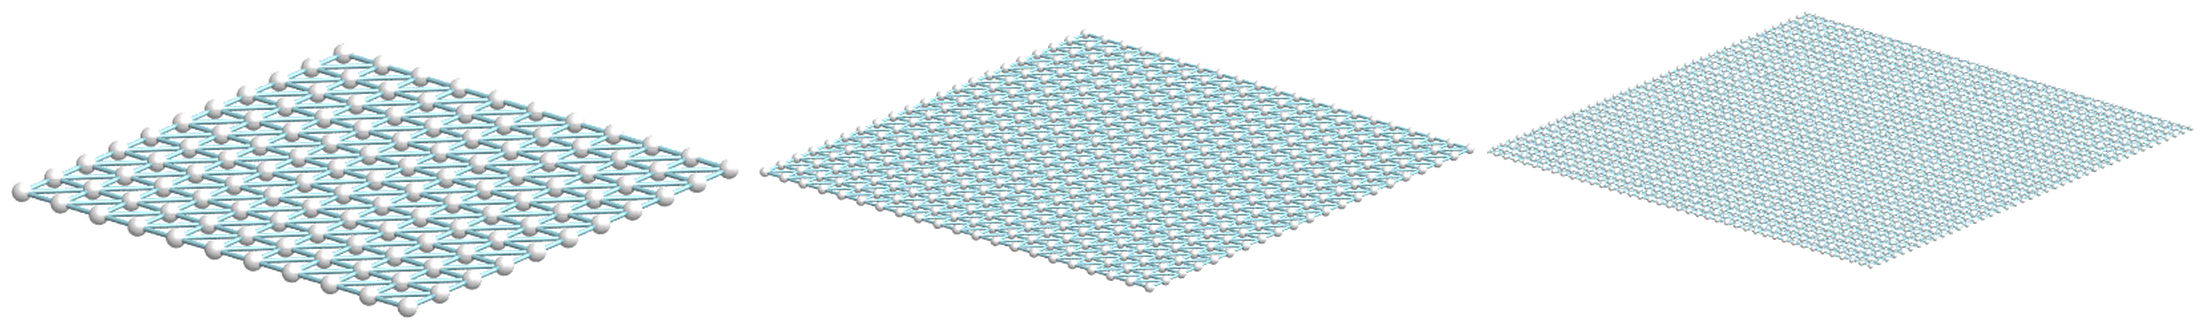
\includegraphics[width=\textwidth]{figs/fig10.png}
\caption{Meshfree discretizations with 36, 121, 441 nodes.}\label{fig:10}
\end{figure}

The normalized support size for quadratic meshfree formulation is set as 2.6.
As shown in Fig. \ref{fig:10}, five regular meshfree discretizations with 36, 121, 441, 1681, 6561 nodes are employed in order to observe the numerical convergence rates of GI and RKGSI.
The convergence performances listed in Figs. \ref{fig:11}--\ref{fig:13} further confirm the theoretical conclusion, which is, when $p=2$, the $L_2$, $H_1$ and $H_2$ errors of RKGSI with $q=p$ respectively converge at the rate of 2, 2 and 1 under refining discretizations, while the convergence rates of GI only achieves about 2, 1 and 0 due to a smaller order of integration consistency than basis function ($q<p$) in traditional Galerkin meshfree methods (such as GI-3, 6 and 9).

\begin{figure}[pos=htbp]
\centering
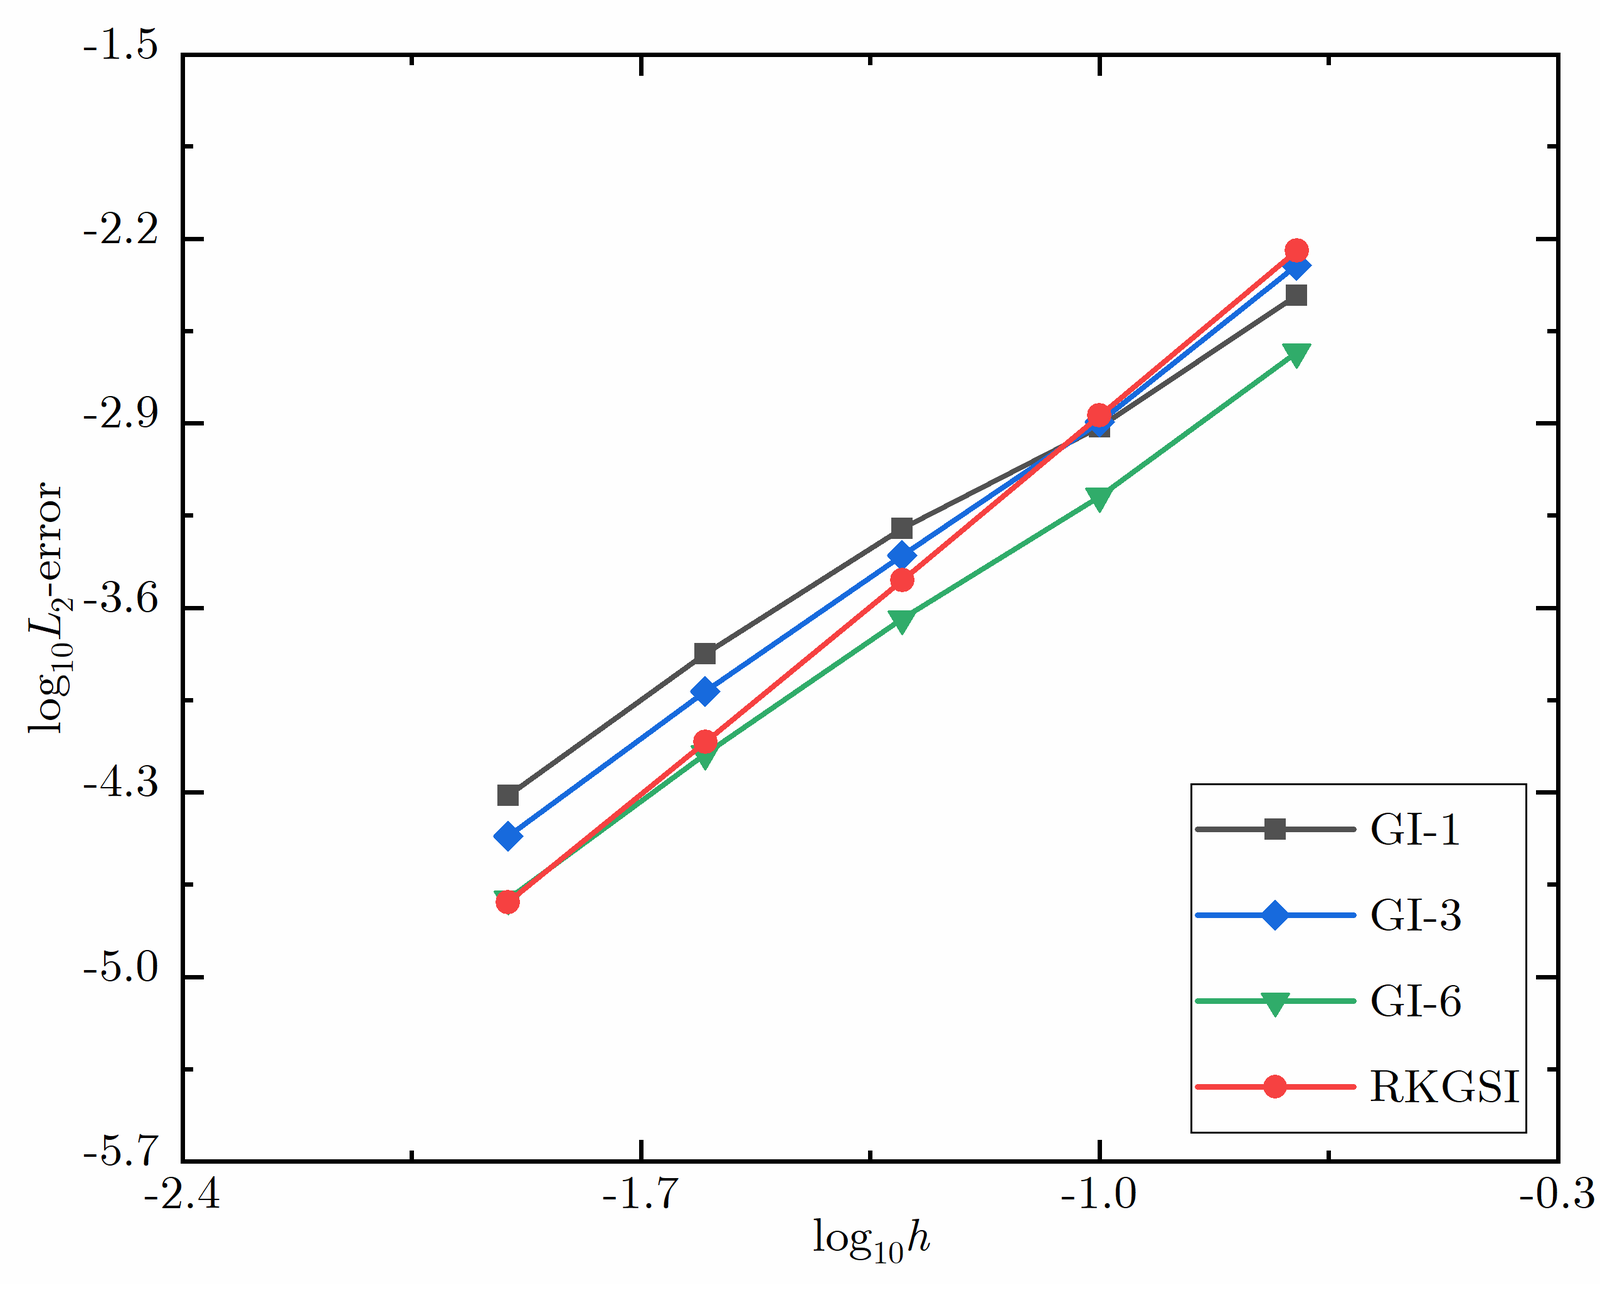
\includegraphics[width=0.55\textwidth]{figs/fig11.png}
\caption{$L_2$-error comparison for the 2D singly clamped plate with $p=2$.}\label{fig:11}
\end{figure}

\begin{figure}[pos=htbp]
\centering
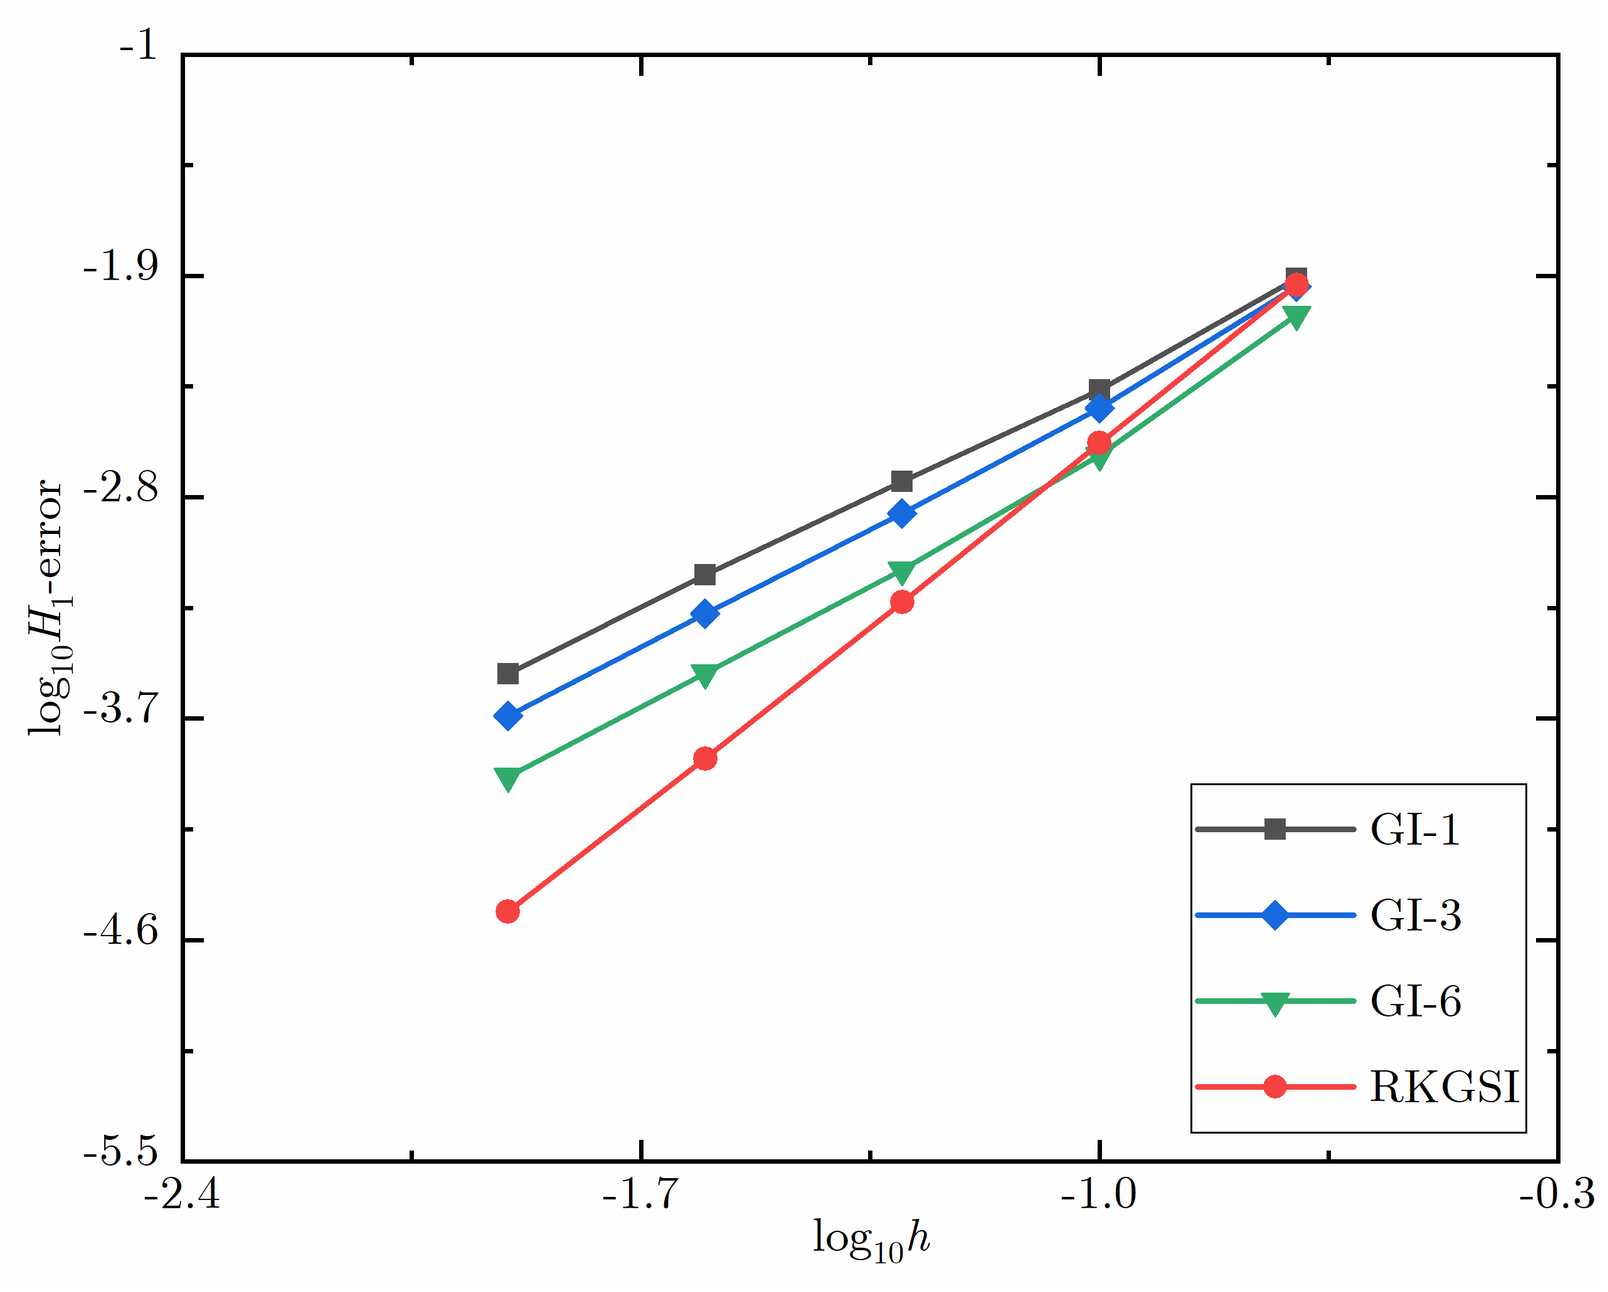
\includegraphics[width=0.55\textwidth]{figs/fig12.png}
\caption{$H_1$-error comparison for the 2D singly clamped plate with $p=2$.}\label{fig:12}
\end{figure}

\begin{figure}[pos=htbp]
\centering
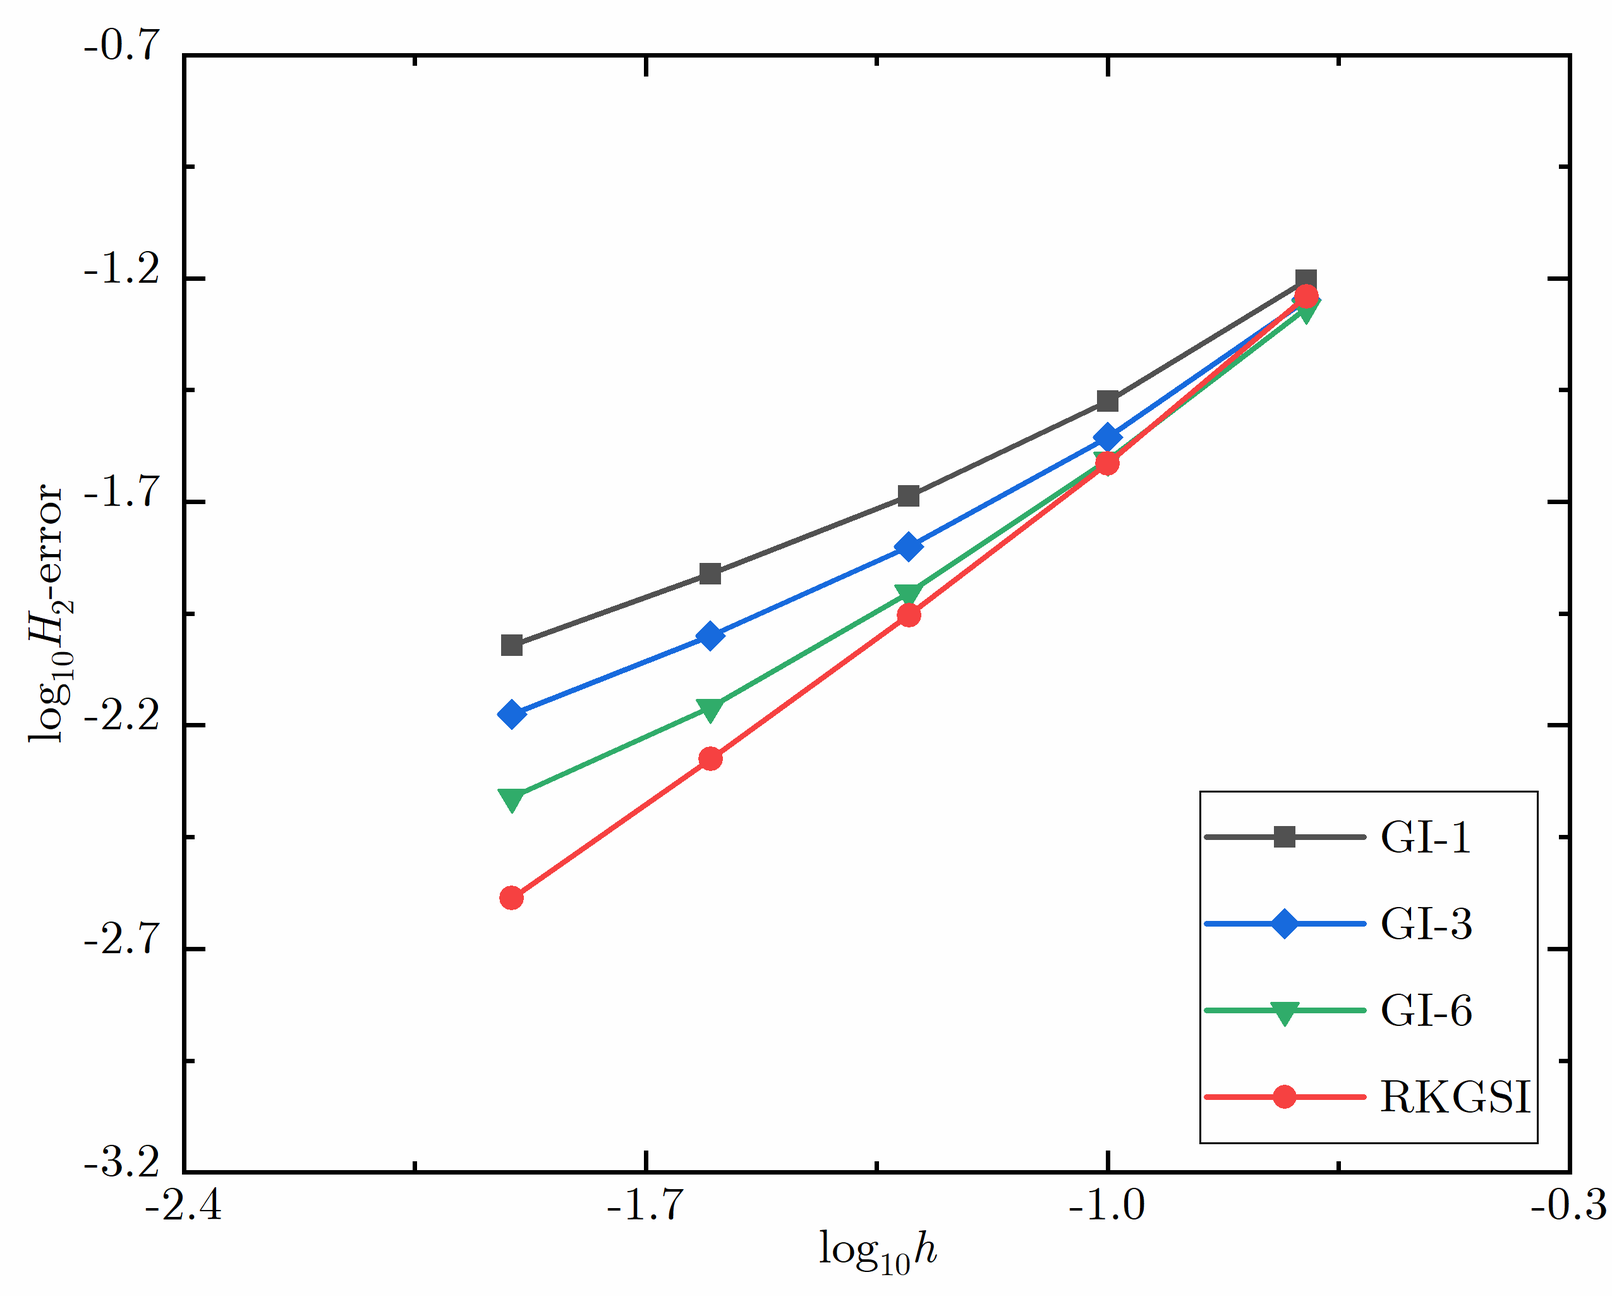
\includegraphics[width=0.55\textwidth]{figs/fig13.png}
\caption{$H_2$-error comparison for the 2D singly clamped plate with $p=2$.}\label{fig:13}
\end{figure}

For better illustrating the importance of integration consistency, in subsequent contents, we will focus on cubic and quartic meshfree formulation with GI and RGKSI.
